\documentclass[../main.tex]{subfiles}

\begin{document}
    \section{Tujuan}
        \begin{enumerate}
            \item Memahami simulasi rangkaian elektronik \textit{buck converter} menggunakan simscape
            \item Melakukan identifikasi model sistem elektronik \textit{buck converter} dengan simscape
        \end{enumerate}
    \section{Dasar Teori}
        \textit{Buck converter} merupakan konverter daya tegangan DC yang dapat menurunkan tegangan ( pada saat yang bersamaan menaikkan arus) dari tegangan input ke tengangan output (load). dalam bentuk konfigurasi umum, sebuah \textit{buck conventer} memilik komponen utama berapa \textit{capacitor} dan \textit{diode} yang digunakan untuk meredam \textit{ripple voltage} dan sebuah \textit{switch}(umumnya mengunakan MOSFET)\cite{Brown}. Blok rangkaian \textit{buck converter} dapat dilihat pada Gambar \ref{buck_converter}.
        \begin{figure}[H]
            \centering
            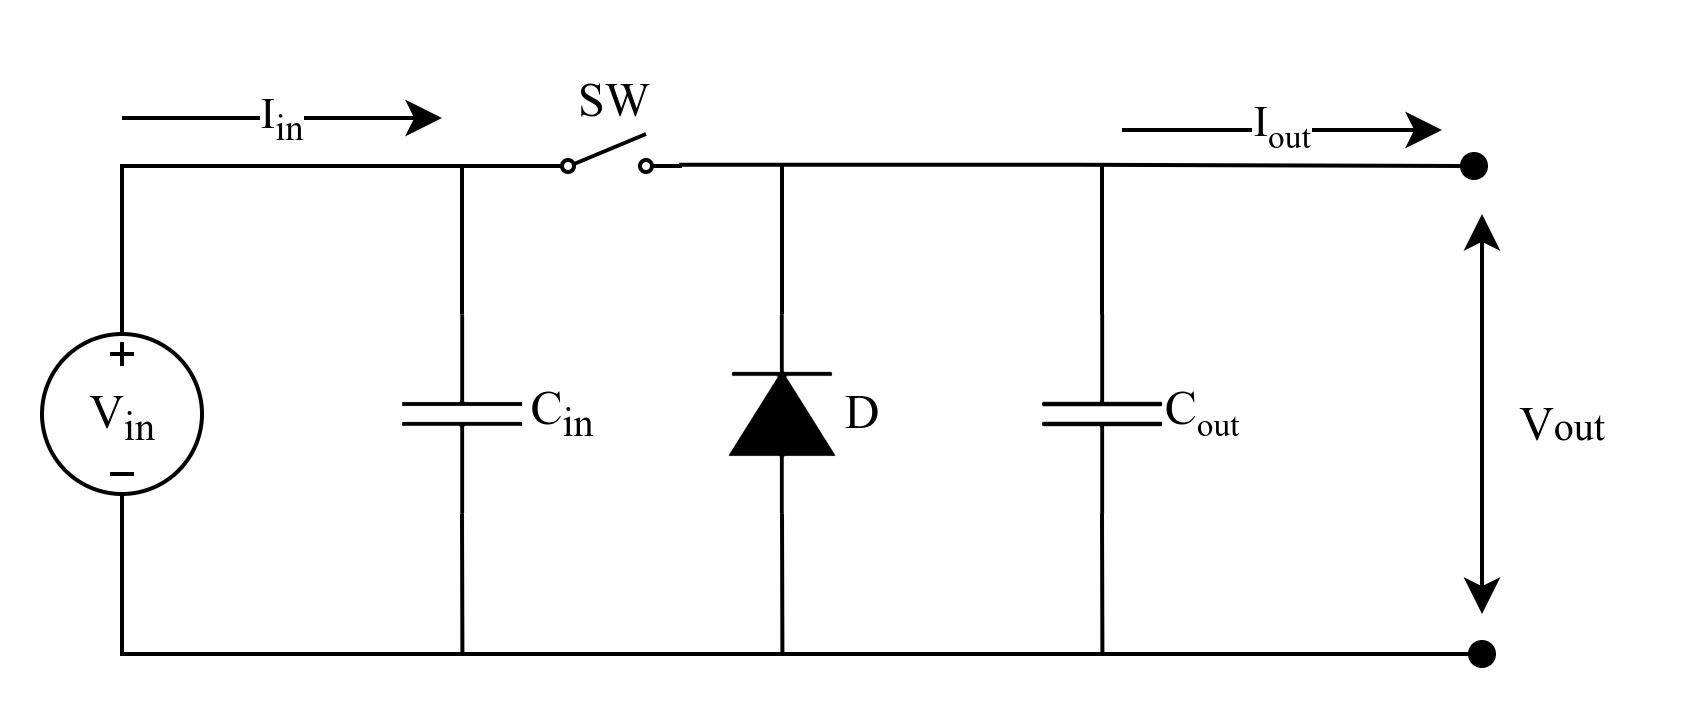
\includegraphics[width = 0.8\textwidth]{assets/image/buck_converter.png}
            \caption{Rangkaian \textit{buck converter}}
            \label{buck_converter}
        \end{figure}
        Dalam pembuatan rangkaian elektronik, diperlukan simulasi untuk mengetahui karakteristrik dan sebagai dasar untuk penalaan sistem. \textit{Simscape} merupakan salah satu perangkat lunak dari MATLAB yang dapat melakukan simulasi rangkaian elektronik. Hasil simulasi rangkaian elektronik dapat dilakukan identifikasi pemodelan menggunakan \textit{system identification toolbox}\cite{Fahmizal}.
    \section{Hasil dan Pembahasan}
        \subsection{Membuat model buck converter pada simscape}
        Dalam melakukan proses identifikasi model pada sistem buck converter, diperlukan simulasi pada model buck converter. simulasi dilakukan menggunakan simscape dengan penyusunan model buck converter ditunjukkan pada Gambar \ref{model_simulink}.
            \begin{figure}[H]
                \centering
                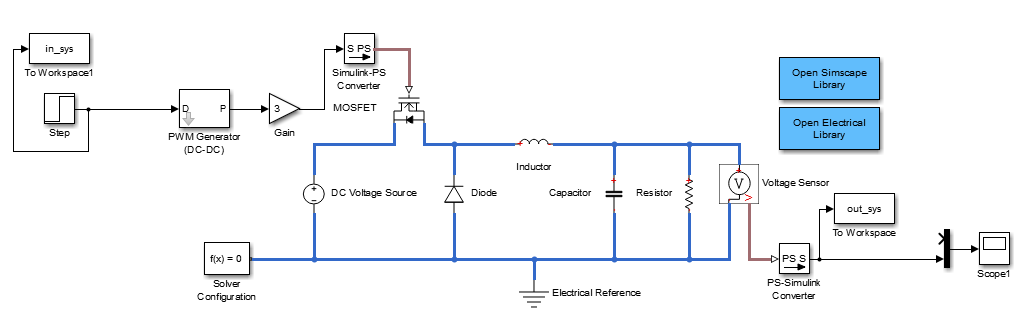
\includegraphics[width = \textwidth]{assets/image/model_simulink.png}
                \caption{Model sistem \textit{buck converter}}
                \label{model_simulink}
            \end{figure}
        Parameter dari masing-masing komponen simulasi rangkaian \textit{buck converter} sebagai berikut,
            \begin{table}[H]
            \centering
            \caption{Parameter simulasi \textit{buck converter} pada simscape}
            \vspace{0.5cm}
            \label{parameter_simulasi}
            \begin{tabular}{|l|l|r|}
            \hline
            \multicolumn{1}{|c|}{\textbf{Komponen}} & \multicolumn{1}{c|}{\textbf{Parameter}}                     & \multicolumn{1}{c|}{\textbf{Nilai}} \\ \hline
            \multirow{4}{*}{Step}          & Step time                                                            & $(1/50000)(100/2)$         \\ \cline{2-3} 
                                           & Initial value                                                        & $0$                        \\ \cline{2-3} 
                                           & Final value                                                          & $0.5$                      \\ \cline{2-3} 
                                           & Sample time                                                          & $0$                        \\ \hline
            \multirow{2}{*}{PWM Generator} & Switching frequency                                                  & $50000$                    \\ \cline{2-3} 
                                           & Sample time                                                          & $0$                        \\ \hline
            Gain                           & Gain                                                                 & $3$                        \\ \hline
            DC Voltage Source              & Constant value DC                                                    & $20$                       \\ \hline
            MOSFET                         & Threshold Voltage                                                    & $2$                        \\ \hline
            \multirow{2}{*}{Inductor}      & Inductance                                                           & $2.00e^{-6}$                  \\ \cline{2-3} 
                                           & Series resistance                                                    & $0.01$                     \\ \hline
            Capacitor                      & Capacitance                                                          & $6.00e^{-5}$                 \\ \hline
            Resistor                       & Resistance                                                           & $1$                        \\ \hline
            \end{tabular}
            \end{table}
            \begin{figure}[H]
                \centering
                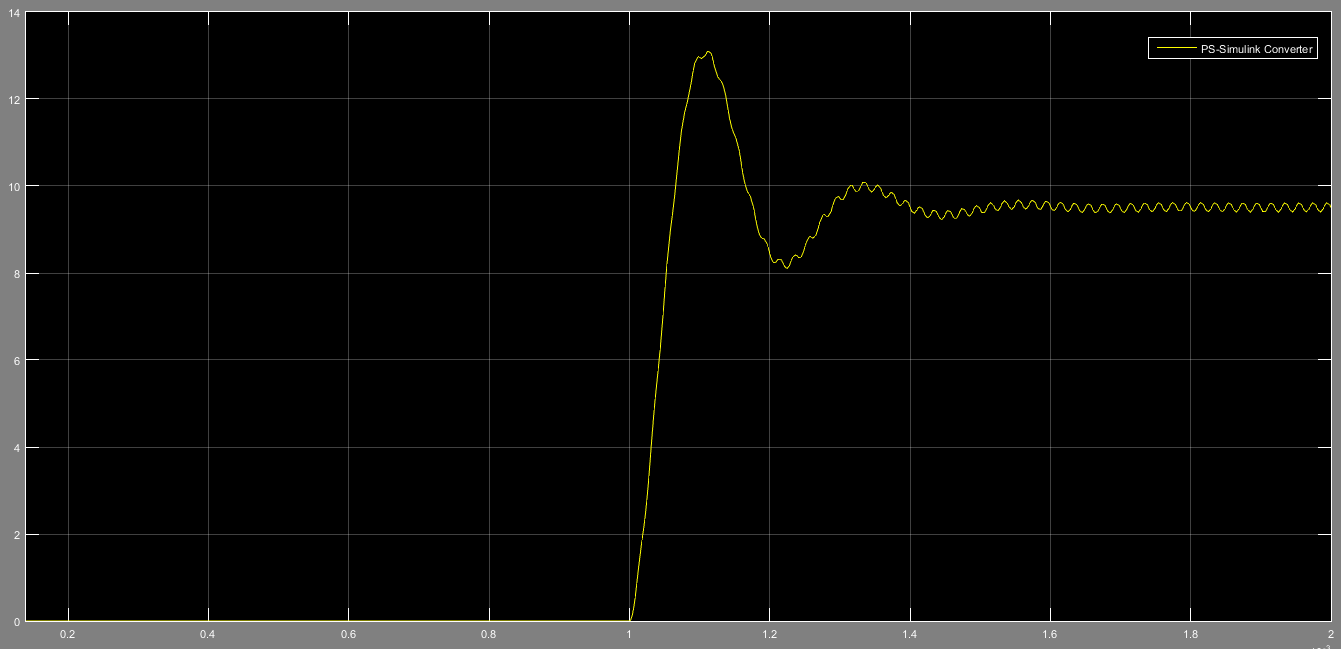
\includegraphics[width = \textwidth]{assets/image/HASIL_SIMULASI_BUCK.png}
                \caption{Hasil simulasi rangkaian \textit{buck converter} pada simscape}
                \label{hasil_simulasi_buck_converter}
            \end{figure}
        \subsection{Identifikasi transfer function sistem}
            Identifikasi sistem dilakukan dengan \textit{system identification toolbox} yang ada di MATLAB. Untuk melakukan identifikasi sistem, data model dari simulasi \textit{buck converter} diolah dengan program berikut,
            \lstinputlisting[language = Matlab]{assets/code/resample.m}
            data yang telah diolah kemudian dilakukan identifikasi dengan pemodelan \textit{transfer fucntion} dengan konfigurasi zero $ = 1$ dan pole $ = 2$. Identifikasi sistem menghasilkan model \textit{transfer function} sebagai berikut,
            \begin{figure}[H]
                \centering
                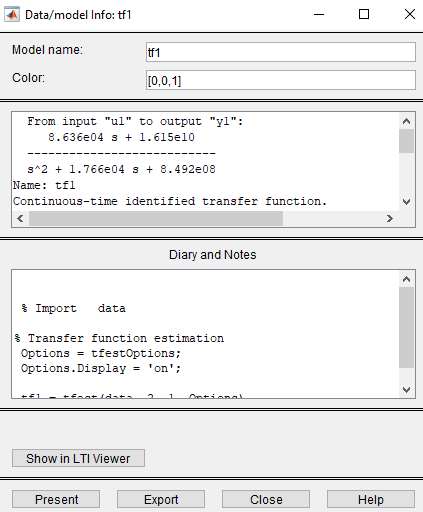
\includegraphics[width = 0.6\textwidth]{assets/image/HASIL_ESTIMASI_MODEL.png}
                \caption{Hasil estimasi sistem menggunakan \textit{system identification toolbox}}
                \label{estimasi_sistem}
            \end{figure}
            Dari hasil estimasi pemodelan \textit{transfer function} dari \textit{system identification toolbox} sebagai berikut,
            \begin{equation}
                G_{(s)} = \frac{8.636e^{4} + 1.615e^{10}}{s^2 + 1.766e^4 + 8.492e^8}
                \label{persamaan_1}
            \end{equation}
            dilakukan perbandingan hasil simulasi simscape dengan hasil identifikasi sistem, didapatkan hasil identifikasi model sistem menggunakan \textit{system identification toolbox} dapat mendekati hasil simulasi menggunakan simscape sebesar $98.98$ seperti yang ditunjukkan pada Gambar \ref{perbandingan_simscape_ident}.
            \begin{figure}[H]
                \centering
                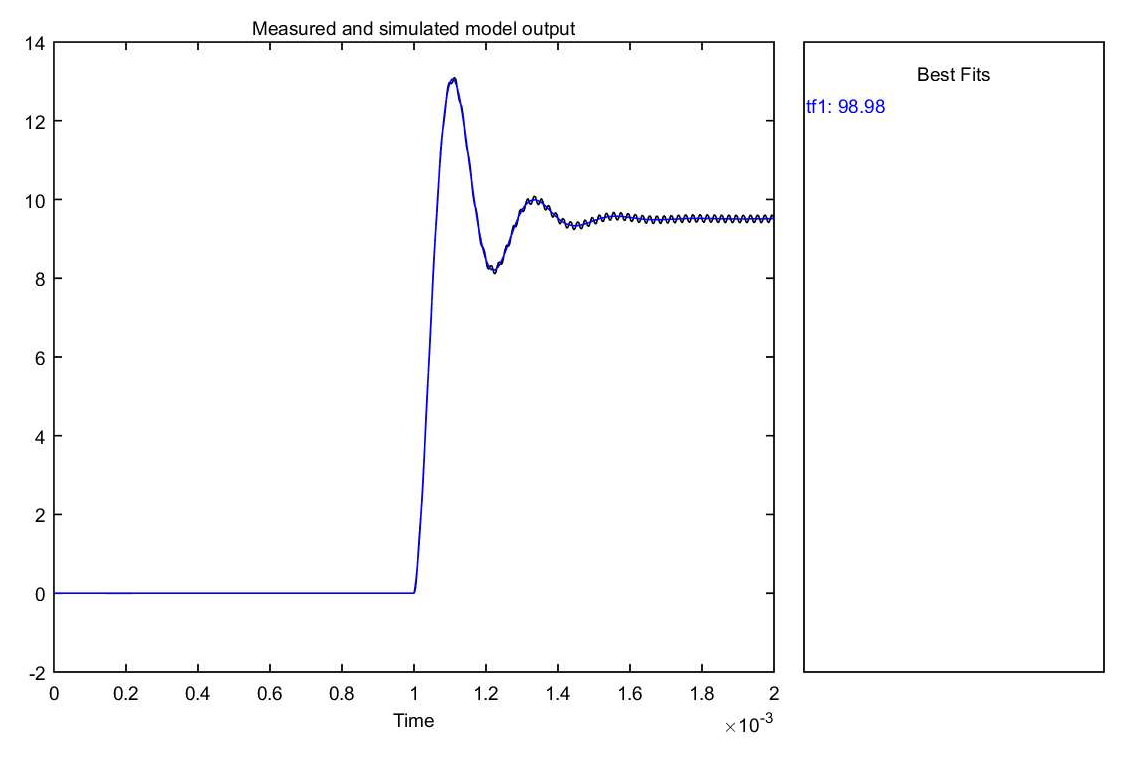
\includegraphics[width = \textwidth]{assets/image/MODEL_OUTPUT-cropped.pdf}
                \caption{Perbandingan hasil estimasi model dan model simulasi \textit{buck converter} pada \textit{system identification toolbox}}
                \label{perbandingan_simscape_ident}
            \end{figure}
        \subsection{Perbandingan hasil simulasi dan identifikasi sistem}
            \begin{figure}[H]
                \centering
                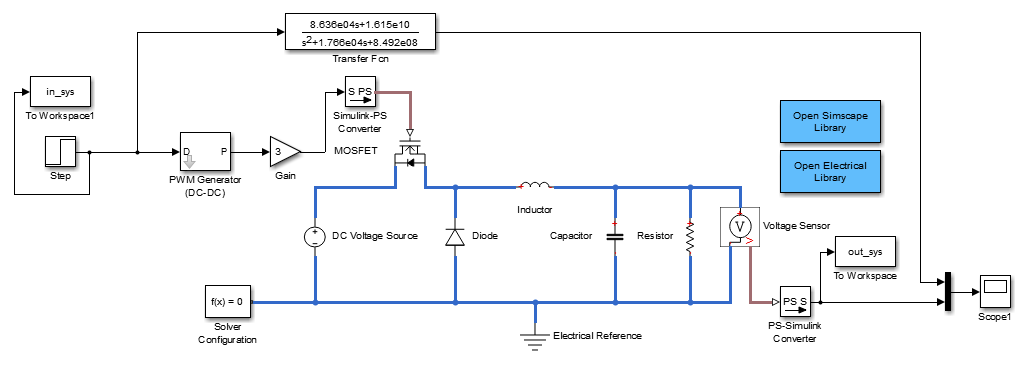
\includegraphics[width = \textwidth]{assets/image/model_simulink_tf.png}
                \caption{Model sistem buck converter dibandingkan dengan hasil estimasi \textit{transfer function}}
                \label{model_simulink_tf}
            \end{figure}
            \begin{figure}[H]
                \centering
                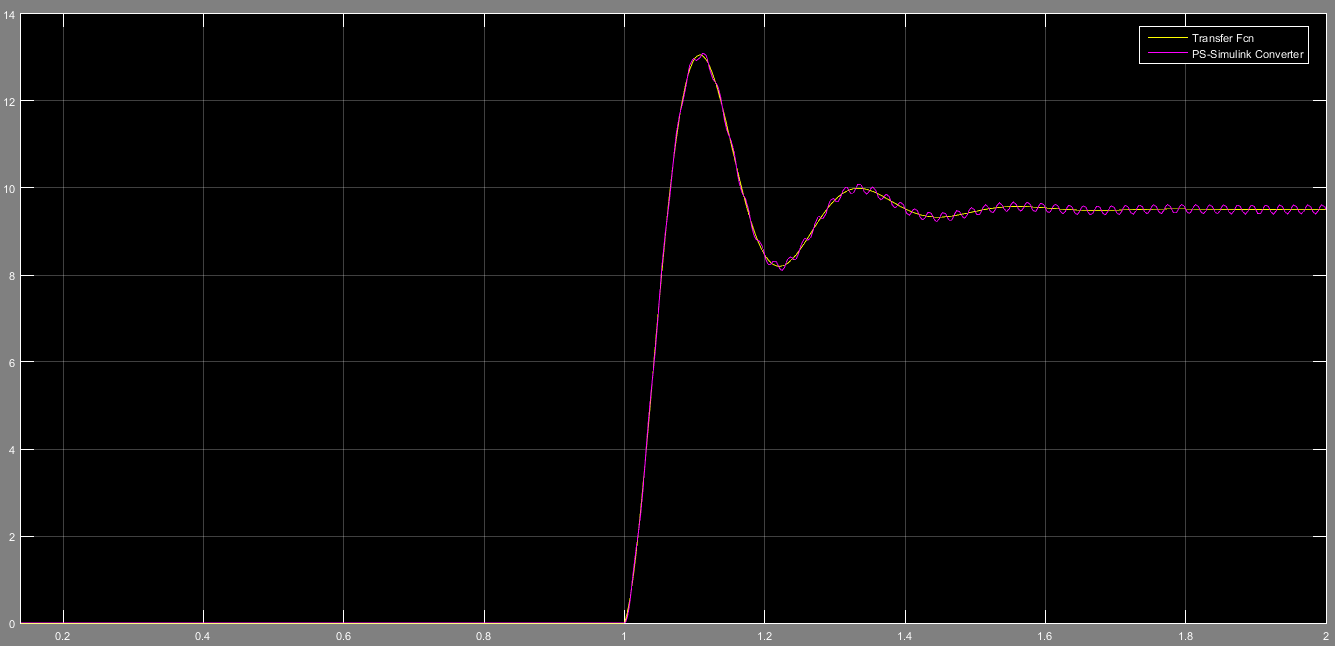
\includegraphics[width = \textwidth]{assets/image/HASIL_PERBADINGAN_MODEL.png}
                \caption{Hasil perbandingan model dari hasil simulasi dan hasil estimasi \textit{transfer function}}
                \label{hasil_perbandingan}
            \end{figure}
            Berdasarkan Gambar \ref{hasil_perbandingan} dapat diamati bahwa hasil estimasi pemodelan \textit{buck converter} memiliki nilai yang mendekati hasil simulasi \textit{buck converter}. Hasil estimasi teramati memiliki garis data yang lebih halus dibandingkan dengan hasil simulasi sistem.
    \section{Kesimpulan}
    Berdasarkan hasil dan pembahasan diatas, didapat kesimpulan sebagai berikut,
    \begin{enumerate}
        \item pemodelan rangkaian elektronik \textit{buck converter} dengan simscape dapat dilakukan dengan membuat rangkaian dan memberikan parameter komponen pada masing-masing komponen simulasi. Data hasil simulasi ditampilkan dalam bentuk plot. 
        \item identifikasi sistem dilakukan dengan \textit{system identification toolbox}, sistem identifikasi sebagai \textit{transfer function} dengan konfigurasi $zero = 1$ dan $pole = 2$. hasil dari identifikasi sistem adalah \textit{transfer function} yang dapat mendekati karakteristik sistem sebesar $98.98$.
    \end{enumerate}
    \pagebreak
    \begin{thebibliography}{1}
        \bibitem[1]{Brown} Brown, M. (2011). Power sources and supplies: World class designs. Elsevier.
        \bibitem[2]{Fahmizal} Fahmizal. 2020. "Identifikasi Sistem Buck Converter menggunakan Simscape" dalam \textit{Modul Praktikum Teknik Kendali Lanjut} (hlm.1-20). Yogyakarta
    \end{thebibliography}
\end{document}